% !TeX root = surprises.tex

\chapter{Are Triangles with Equal Areas and Perimeters Congruent?}\label{c.congruent}

%%%%%%%%%%%%%%%%%%%%%%%%%%%%%%%%%%%%%%%%%%%%%%%%%%%%%%%%%%%%%%%

\abstract*{Are triangles with the equal area and equal perimeter congruent? Not necessarily: the triangles with sides $(17,25,28)$ and $(20,21,29)$ both have perimeter $70$ and area $210$, but are not congruent. This chapter shows that given a triangle with rational sides, it is possible to construct a non-congruent triangle with rational sides which has the same area and perimeter. We carry out the derivation using an example by showing that the triangle with sides $(3,4,5)$ and the triangle with sides  $\left(\frac{156}{35}, \frac{101}{21}, \frac{41}{15}\right)$ both have perimeter $12$ and area $6$.}

%%%%%%%%%%%%%%%%%%%%%%%%%%%%%%%%%%%%%%%%%%%%%%%%%%%%%%%%%%%%%%%

Are two triangles with the same area and the same perimeter congruent? Not necessarily:\index{Triangle!same area and perimeter} the triangles with sides $(17,25,28)$ and $(20,21,29)$ both have perimeter $70$ and area $210$, but they are  not congruent (Fig.~\ref{f.congruent-first-example}).\footnote{The areas were computed using Heron's formula\index{Triangle!Heron's formula} (Thm.~\ref{thm.heron}) and the angles using the Law of Cosines\index{Law of cosines} (Thm.~\ref{thm.law-of-cosines}).} This chapter shows that given a triangle with rational sides it is possible to construct a non-congruent triangle also with rational sides that has the same area and the perimeter.
We carry out the derivation using an example, showing that the triangle with sides $(3,4,5)$ and the triangle with sides 
$\left(\frac{156}{35}, \frac{101}{21}, \frac{41}{15}\right)$ both have perimeter $12$ and area $6$.

\begin{figure}[b]
\begin{center}
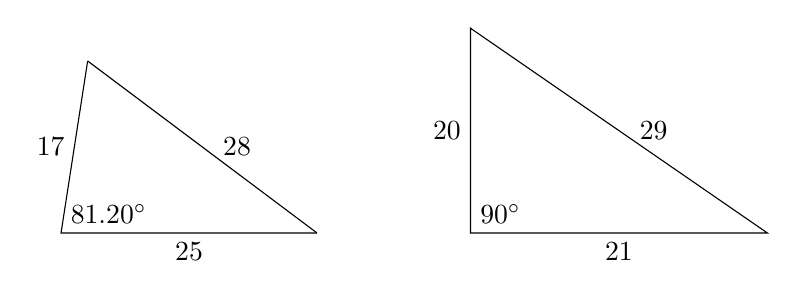
\begin{tikzpicture}[scale=1.3]
\coordinate (A1) at (0,0);
\node[above right] at (A1) {$81.20^\circ$};
\coordinate (B1) at (2.5cm,0);
\coordinate (C1) at (81.20:1.7cm);
\draw (B1) -- node[below] {$25$} (A1) -- node[left] {$17$} (C1);
\draw (B1) -- node[right,xshift=4pt] {$28$} +(143.13:2.8cm);
\begin{scope}[xshift=4cm]
\coordinate (A2) at (0,0);
\node[above right] at (A2) {$90^\circ$};
\coordinate (B2) at (2.9cm,0);
\coordinate (C2) at (0,2cm);
\draw (B2) -- node[below] {$21$} (A2) -- node[left] {$20$} (C2) -- node[right,xshift=4pt] {$29$} cycle;
\end{scope}
\end{tikzpicture}
\end{center}
\caption{Non-congruent triangles with the same area and the same perimeter}\label{f.congruent-first-example}
\end{figure}


\section{From a Triangle to an Elliptic Curve}\label{s.elliptic}

The three angle bisectors in a triangle intersect in a point called the \emph{incenter}\index{Triangle!incenter} of the triangle. The incenter is the center of a circle inscribed\index{Inscribed circle} within the triangle  (Fig.~\ref{f.congruent1}). 

Drop altitudes from $O$ to the sides. The altitudes have length $r$, the radius of the inscribed circle. The altitudes and angle bisectors create three pairs of congruent right triangles:
\[
\triangle AOB'\cong \triangle AOC',\quad \triangle BOA'\cong \triangle BOC',\quad \triangle COA'\cong \triangle COB'\,.
\]

\begin{figure}[t]
\begin{center}
\begin{tikzpicture}[scale=1.85]
% Draw base and path two lines at known angles
\draw (0,0) coordinate (a) node[below] {$A$} -- (0:6) coordinate (b) node[below] {$B$};
\path[name path=ac] (a) -- +(50:4);
\path[name path=bc] (b) -- +(150:5);
% Get their intersection and draw lines between vertices
\path[name intersections={of=ac and bc,by=c}];
\node[above] at (c) {$C$};
\draw (a) -- (c) -- (b) -- (a);
% Label angles with tick marks
\draw (a) ++(0:4mm) arc (0:50:4mm);
\draw (a) ++(10:3.5mm) -- +(10:1mm);
\draw (a) ++(15:3.5mm) -- +(15:1mm);
\draw (a) ++(35:3.5mm) -- +(35:1mm);
\draw (a) ++(40:3.5mm) -- +(45:1mm);
\draw (b) ++(150:5mm) arc (150:180:5mm);
\draw (b) ++(157.5:4.5mm) -- +(157.5:1mm);
\draw (b) ++(172.5:4.5mm) -- +(172.5:1mm);
\draw (c) ++(230:3mm) arc (230:330:3mm);
\draw (c) ++(250:2.5mm) -- +(250:1mm);
\draw (c) ++(255:2.5mm) -- +(255:1mm);
\draw (c) ++(260:2.5mm) -- +(260:1mm);
\draw (c) ++(300:2.5mm) -- +(300:1mm);
\draw (c) ++(305:2.5mm) -- +(305:1mm);
\draw (c) ++(310:2.5mm) -- +(310:1mm);
% Path bisectors of two lines
\path[name path=bia] (a) -- +(25:3.5);
\path[name path=bib] (b) -- +(165:5);
% Intersection of angle bisectors
\path [name intersections={of=bia and bib,by=center}];
% Draw angle bisectors to center
\draw (a) -- (center);
\draw (c) -- (center);
\draw (b) -- (center);
% Draw radii
\draw (center) -- node[left] {$r$} ($(a)!(center)!(b)$) node[below,yshift=-2pt] {$C'$} coordinate (ap);
\draw (center) -- node[left,yshift=-4pt] {$r$} ($(a)!(center)!(c)$) node[above left,xshift=4pt] {$B'$} coordinate (bp);
\draw (center) -- node[right] {$r$} ($(b)!(center)!(c)$) node[above right] {$A'$} coordinate (cp);
\vertex{center};
\node[above,xshift=3pt,yshift=6pt] at (center) {$O$};
% Draw right angle squares
\draw (ap) -- ++(90:4pt) -- ++(0:4pt) -- ++(-90:4pt);
\draw (bp) -- ++(-40:4pt) -- ++(-130:4pt) -- ++(-220:4pt);
\draw (cp) -- ++(-30:4pt) -- ++(-120:4pt) -- ++(-210:4pt);
% Labels of angles
\node[above,xshift=5pt,yshift=21pt] at (center) {$\gamma/2$};
\node[above left,xshift=-4pt,yshift=21pt] at (center) {$\gamma/2$};
\node[above right,xshift=4pt,yshift=-5pt] at (center) {$\beta/2$};
\node[below right,yshift=-6pt] at (center) {$\beta/2$};
\node[left,xshift=-8pt,yshift=3pt] at (center) {$\alpha/2$};
\node[below left,xshift=2pt,yshift=-6pt] at (center) {$\alpha/2$};
% Labels of line segments (names of points are weird...)
\path (a) -- node[below,yshift=-2pt] {$u$} (ap);
\path (a) -- node[left, xshift=-2pt] {$u$} (bp);
\path (b) -- node[above,yshift=2pt]  {$v$} (cp);
\path (b) -- node[below,xshift=-2pt] {$v$} (ap);
\path (c) -- node[above,xshift=-2pt] {$w$} (bp);
\path (c) -- node[above,xshift=2pt]  {$w$} (cp);
% Labels of sides
\draw[<->] ($(a)+(0,-10pt)$) -- node[fill=white] {$c$} 
           ($(b)+(0,-10pt)$);
\draw[<->] ($(a)+(-4pt,7pt)$) -- node[fill=white] {$b$}
           ($(c)+(-4pt,7pt)$);
\draw[<->] ($(b)+(2pt,9pt)$) -- node[fill=white] {$a$}
           ($(c)+(2pt,9pt)$);
% Inscribed circle
\node[draw,circle through=(ap)] at (center) {};
\end{tikzpicture}
\end{center}
\caption{The incenter of a triangle}\label{f.congruent1}
\end{figure}

The altitudes divide the sides $a,b,c$ into segments $u,v,w$. Denote the central angles at $O$ by $\alpha/2,\beta/2,\gamma/2$.
The area of $\triangle ABC$ is the sum of the areas of $\triangle BOC, \triangle AOB, \triangle AOC$:
%
\begin{subeqnarray}
A &=& \frac{1}{2}(w+v)r + \frac{1}{2}(v+u)r + \frac{1}{2}(u+w)r\\
&=&\frac{1}{2}\cdot 2(u+v+w)r\\
&=&\frac{1}{2}(a+b+c)r\\
&=&sr\,, \slabel{eq.area1}
\end{subeqnarray}
where $s$ is the \emph{semi-perimeter}, one-half the perimeter of the triangle $\triangle ABC$. The lengths of $u,v,w$ can be expressed using the central angles and the radius of the circle:
\begin{align}
\tan \frac{\alpha}{2}= \frac{u}{r},\quad
\tan \frac{\beta}{2} = \frac{v}{r},\quad
\tan \frac{\gamma}{2} =\frac{w}{r}\,.\label{eq.uvw}
\end{align}

\newpage

The semi-perimeter can now be expressed in terms of the tangents:
\[
s = u+v+w = r\tan \frac{\alpha}{2}+r\tan \frac{\beta}{2}+r\tan \frac{\gamma}{2} = r\left(\tan \frac{\alpha}{2}+\tan \frac{\beta}{2}+\tan \frac{\gamma}{2}\right)\,,
\]
and by Eq.~\ref{eq.area1} the area is:
\begin{align}
A = sr = r^2\left(\tan \frac{\alpha}{2}+\tan \frac{\beta}{2}+\tan \frac{\gamma}{2}\right)\,.\label{eq.area2}
\end{align}
From $r=A/s$ Eq.~\ref{eq.area2} can be written as:
\begin{align}
\tan \frac{\alpha}{2}+\tan \frac{\beta}{2}+\tan \frac{\gamma}{2} = \frac{A}{r^2} = \frac{A}{(A/s)^2} = \frac{s^2}{A}\,.\label{eq.area3}
\end{align}
Since the sum of the angles $\alpha,\beta,\gamma$ is $360^\circ$:
%
\begin{subeqnarray}
\gamma/2 &=& 360^\circ/2 - (\alpha/2 + \beta/2)\\
\tan\gamma/2 &=& \tan(180^\circ - (\alpha/2 + \beta/2))\\
 &=& -\tan (\alpha/2 + \beta/2)\\
&=& \frac{\tan\alpha/2 + \tan\beta/2}{\tan\alpha/2 \, \tan\beta/2-1}\,,\slabel{eq.tangent1}
\end{subeqnarray}
using the formula for the tangent of the sum of two angles (Thm.~\ref{thm.tangent-sum}).

Let us simplify the notation by defining variables for the tangents:
\begin{align}
x=\tan \frac{\alpha}{2},\quad
y=\tan \frac{\beta}{2},\quad
z=\tan \frac{\gamma}{2}\,.\label{eq.variables-for-tangents}
\end{align}
By Eq.~\ref{eq.tangent1} we can express $z=\tan\gamma/2$ in terms of $x,y$:
\begin{align}
z = \frac{x+y}{xy-1}\,.\label{eq.xy1}
\end{align}
With this notation, Eq.~\ref{eq.area3} becomes:
\begin{align}
x+y+\frac{x+y}{xy-1}=\frac{s^2}{A}\,.\label{eq.xy2}
\end{align}
Given fixed values of $A$ and $s$, are there multiple solutions of Eq.~\ref{eq.xy2}?

For the right triangle $(3,4,5)$:
\begin{align}
\frac{s^2}{A} = \frac{\left(\frac{1}{2}(3+4+5)\right)^2}{\frac{1}{2}\cdot 3\cdot 4} = \frac{6^2}{6}=6\,.
\end{align}

\newpage

\noindent{}If there is another solution Eq.~\ref{eq.xy2} with $s^2/A=6$, it can be written as:
\begin{subeqnarray}
x+y+\frac{x+y}{xy-1}&=&6\\
x^2y + xy^2 -6xy + 6 &=& 0\,.\slabel{eq.elliptic}
\end{subeqnarray}
This is an equation for an \emph{elliptic curve}\index{Elliptic curve}.

\section{Solving the Equation for the Elliptic Curve}

A portion of the graph of Eq.~\ref{eq.elliptic} is shown Fig.~\ref{f.two-secants}. Any point on the closed curve in the first quadrant is a solution to the equation because the lengths of the sides of the triangle must be positive. $A,B,D$ correspond to the triangle $(3,4,5)$ as shown below. To find additional rational solutions the \emph{method of two secants} is used.\index{Two secants, method of}

Construct a secant through the points $A=(2,3), B=(1,2)$. It intersects the curve at $C=(-1.5,-0.5)$, but this does not give a solution because the values are negative. Construct a second secant from $C$ to $D=(3,2)$. The intersection with the curve at $E\approx (1.5,1.2)$ does give a new solution whose coordinates will be computed below.

\begin{figure}[t]
\begin{center}
\begin{tikzpicture}[scale=1.2]
\draw[very thin,step=10mm] (-4,-4) grid (4,4);
\draw[thick] (-4,0) -- (4,0);
\draw[thick] (0,-4) -- (0,4);
\foreach \x in {-3,...,4}
  \node at (\x-.2,-.2) {\sm{\x}};
\foreach \y in {-3,...,-1}
  \node at (+.2,\y-.3) {\sm{\y}};
\foreach \y in {1,...,4}
  \node at (+.2,\y-.3) {\sm{\y}};

\draw[very thick,domain=.936:3.306,samples=200] plot (\x,{
(
  (6*\x-\x*\x)+
  sqrt(
   (\x*\x-6*\x)^2 -
   4*\x*6
  )
)/
(2*\x)
});

\draw[very thick,domain=.936:3.306,samples=100] plot (\x,{
(
  (6*\x-\x*\x)-
  sqrt(
   (\x*\x-6*\x)^2 -
   4*\x*6
  )
)/
(2*\x)
});

\draw[very thick,domain=-2.5:-.25,samples=100] plot (\x,{
(
  (6*\x-\x*\x)+
  sqrt(
   (\x*\x-6*\x)^2 -
   4*\x*6
  )
)/
(2*\x)
});

\coordinate (A) at (2,3);
\coordinate (B) at (1,2);
\coordinate (C) at (-1.5,-0.5);
\coordinate (D) at (3,2);
\coordinate (E) at (1.5,1.2);

\draw[very thick,dashed,red]  ($(C)!-.4!(A)$) -- ($(C)!1.2!(A)$);
\draw[very thick,dashed,blue] ($(C)!-.4!(D)$) -- ($(C)!1.2!(D)$);

\node[right,xshift=8pt,yshift=-2pt] at (A) {$A=(2,3)$};
\node[above left,xshift=2pt] at (B) {$B=(1,2)$};
\node[right,xshift=20pt,yshift=-4] at (C)  {$C=(-1.5,-0.5)$};
\node[right,xshift=6pt,yshift=-6pt] at (D) {$D=(3,2)$};
\node[below,xshift=8pt,yshift=-12pt] at (E) {$E=(1.5,1.2)$};

\end{tikzpicture}
\end{center}
\caption{The method of two secants}\label{f.two-secants}
\end{figure}


The equation of the (red) line through $A,B$ is $y=x+1$. From Eq.~\ref{eq.elliptic}:
\begin{eqnarray*}
x^2(x+1) + x(x+1)^2 -6x(x+1) +6 &=&0\\
2x^3 -3x^2 -5x +6 &=&0\,.
\end{eqnarray*}
From $A,B$ we know two roots $x=2,x=1$ so we can factor the cubic polynomial:
\[
(x-2)(x-1)(ax+b)=0\,,
\]
where the third root is unknown. Multiply the factors and conclude that $a=2, b=3$ since $2x^3 -3x^2 -5x +6 = ax^3+\cdots+2b$. The third factor is $2x+3$ which gives the third root $x=-\frac{3}{2}$ and $y=x+1=-\frac{1}{2}$. This is the point $C=(-\frac{3}{2},-\frac{1}{2})$ in the graph.

The equation of the (blue) line through $C,D$ is:
\begin{align}
y = \frac{5}{9}x + \frac{1}{3}\,.\label{eq.second-secant}
\end{align}
Substitute for $y$ in Eq.~\ref{eq.elliptic}:
\begin{eqnarray*}
x^2\left(\frac{5}{9}x + \frac{1}{3}\right) + x\left(\frac{5}{9}x + \frac{1}{3}\right)^2 -6x\left(\frac{5}{9}x + \frac{1}{3}\right) +6 &=&0\\
\frac{70}{81}x^3 - \frac{71}{27}x^2 - \frac{17}{9}x +6 &=&0\,.
\end{eqnarray*}
From $C,D$ we know two roots $x=3,x=-\frac{3}{2}$ so we can factor the cubic polynomial:
\[
(x-3)\left(x+\frac{3}{2}\right)(ax+b)=0\,.
\]
Equating the coefficients of the cubic term and the constant terms gives:
\begin{eqnarray*}
\frac{70}{81}x - \frac{4}{3}&=&0\\
x&=& \frac{54}{35}\approx 1.543\,,
\end{eqnarray*}
and $y$ can be computed from Eq.~\ref{eq.second-secant}:
\[
y=\frac{25}{21}\approx 1.190\,.
\]

\newpage

The coordinates of $E$ are:
\[
\left(\frac{54}{35}, \frac{25}{21}\right)=(1.543,1.190)\,,
\]
which are close to the approximations $(1.5,1.2)$ obtained from the graph.

Finally, compute $z$ from Eq.~\ref{eq.xy1}:
\[
z=\frac{x+y}{xy-1}=%
\displaystyle\left(\frac{54}{35} + \frac{25}{21}\right)%
 \, \bigg/ \,%
\displaystyle\left(\frac{54}{35}\frac{25}{21}-1\right)=%
\frac{2009}{615} = \frac{49}{15}\,.
\]

\section{Derivation of a Triangle From the Elliptic Curve}

\enlargethispage*{\baselineskip}

Using Eqs.~\ref{eq.uvw}, ~\ref{eq.variables-for-tangents}, $a,b,c$, the sides of the triangle $\triangle ABC$, can be computed from $x,y,z$ and $r=A/s=6/6=1$:
%
\begin{eqnarray*}
a&=&w+v = r(z+y)=(z+y)\\
b&=&u+w= r(x+z)=(x+z)\\
c&=&u+v=r(x+y)=(x+y)\,.
\end{eqnarray*}
For solution $A$ of the elliptic curve the sides of the triangle are:
\begin{eqnarray*}
a &=& z+y = 1+3 = 4\\
b &=& x+z = 2+1=3\\
c &=& x+y = 2+3=5\,.
\end{eqnarray*}
For solution $E$ of the elliptic curve the sides of the triangle are:
\begin{eqnarray*}
a &=& z+y = \frac{49}{15} + \frac{25}{21} = \frac{156}{35}\\
&&\\
b &=& x+z = \frac{54}{35} + \frac{49}{15} = \frac{101}{21}\\
&&\\
c &=& x+y = \frac{54}{35} + \frac{25}{21} =\frac{41}{15}\,.
\end{eqnarray*}
Let us check this result. The semi-perimeter is:
\[
s=\frac{1}{2}\left(\frac{156}{35} + \frac{101}{21}+\frac{41}{15}\right) = \frac{1}{2}\left(\frac{468+505+287}{105}\right) = \frac{1}{2}\left(\frac{1260}{105}\right)= 6\,,
\]

\newpage

\noindent{}and the area can be computed using Heron's formula\index{Heron's formula|see {Triangle, Heron's formula}} (Thm.~\ref{thm.heron}):
\[
A= \sqrt{6 \left(6-\frac{156}{35}\right) \left(6-\frac{101}{21}\right) \left(6-\frac{41}{15}\right)}=\sqrt{36} = 6\,.
\]
Is $\left(\frac{156}{35}, \frac{101}{21}, \frac{41}{15}\right)\cong(3,4,5)$? To simplify the computation let us use the decimal approximations $(4.48,4.81,2.73)$. Then:
\[
\sqrt{4.48^2+2.73^2}=5.25\neq 4.81\,,
\]
so this is not a right triangle and not congruent to $(3,4,5)$.
We can use the Law of Cosines to compute an angle and construct the triangle (Fig.~\ref{f.not-a-right-triangle}):
\[
\cos^{-1}\left((4.48^2+2.73^2 - 4.81^2)/(2\cdot 4.48\cdot 2.73)\right)\approx 79.67^\circ\,.
\]

\begin{figure}[t]
\begin{center}
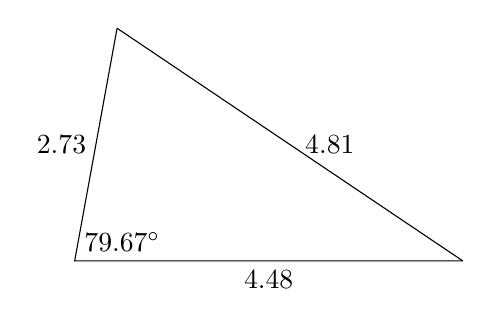
\begin{tikzpicture}[scale=1.1]
\coordinate (A1) at (0,0);
\node[above right] at (A1) {$79.67^\circ$};
\coordinate (B1) at (4.48cm,0);
\coordinate (C1) at (79.67:2.73cm);
\draw (B1) -- node[below] {$4.48$} (A1) -- node[left] {$2.73$} (C1);
\draw (B1) -- node[right,xshift=2pt] {$4.81$} (C1);
\end{tikzpicture}
\end{center}
\caption{$\left(\frac{156}{35}, \frac{101}{21}, \frac{41}{15}\right)$ is not a right triangle}\label{f.not-a-right-triangle}
\end{figure}

\vspace{-4ex}

\subsection*{What Is the Surprise?}

Are triangles with the same area and perimeter congruent? My first impression was to say ``yes,'' because it is not easy to find counterexamples. What is surprising is that given an arbitrary triangle with rational sides, it is possible to construct a non-congruent triangle with rational sides which has the same area and perimeter, although the result can be strange as with the triangles $(3,4,5)$ and $\left(\frac{156}{35}, \frac{101}{21}, \frac{41}{15}\right)$.

\vspace{-2ex}

\subsection*{Sources}

This chapter is based on \cite{mccallum}. In \cite{marita} it is shown that given an isoceles triangle there are non-congruent triangles with the same area and perimeter, but the proof does not include an explicit construction.
